%\subsection{Существующие подходы}

\begin{frame}{Полный перебор}
В 1913 году в работе Цермело\footnotemark{} было доказано существование оптимальной стратегии игры с полной информацией.
Подход состоит в построении полного дерева игры.
\begin{figure}
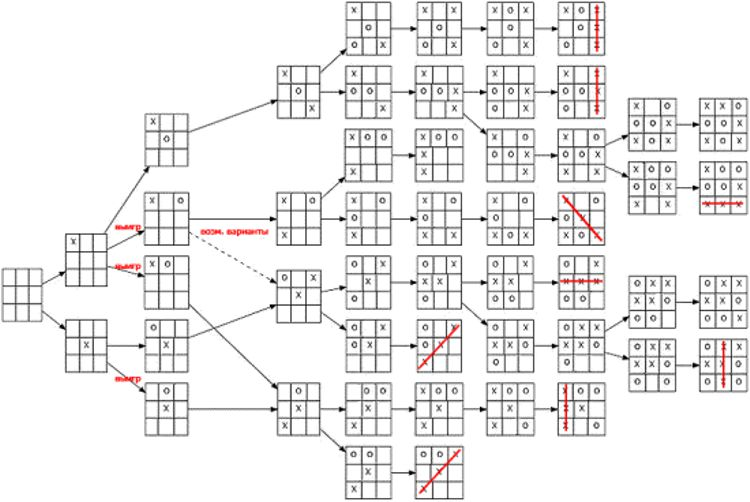
\includegraphics[scale=0.3]{./pictures/xoxo.jpg}
\end{figure}
\footnotetext{Е. Zermelо, Obereine Anwendung der Mengenlehre attfdie Theorie des Schachspiels (Cambridge, 1913)}
%Zermelo E. Über eine Anwendung der Mengenlehre auf die Theorie des Schachspiels //Proceedings of the fifth international congress of mathematicians. – II, Cambridge UP, Cambridge, 1913. – Т. 2. – С. 501-504.
\end{frame}

%\begin{frame}{Полное дерево игры}
%\begin{figure}
%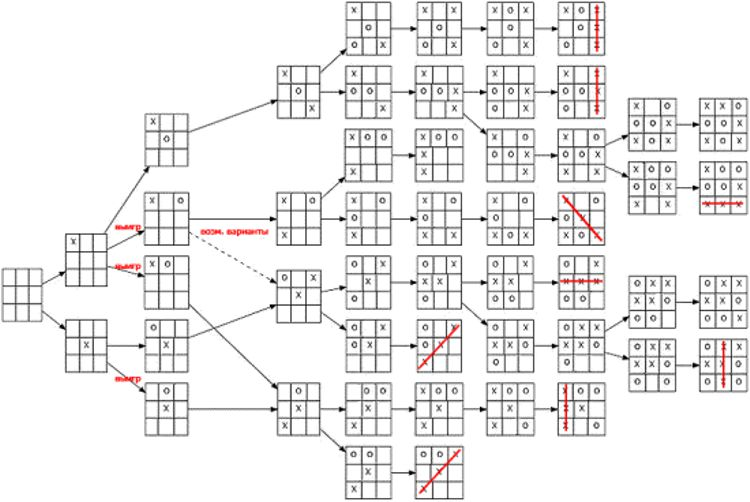
\includegraphics[scale=0.5]{./pictures/xoxo.jpg}
%\end{figure}
%\end{frame}

\begin{frame}{Особенности переборного подхода}
\begin{itemize}
\item После $m$ ходов дерево игры содержит порядка $d^m$ листов, где $d$ -- среднее количество возможных ходов в позиции.
\item Для крестиков-ноликов $d \approx 5$, для шахмат $d \approx 60$, для~го~$d \approx 400$. 
\item Построение требует большой вычислительной мощности.
\item Включает в себя множество очевидно бессмысленных ходов.
\item Проводится сокращение дерева с помощью различных эвристических методов (minimax, alpha-beta и другие).
\item У современных программ, с учетом отсечений, осуществляется перебор $100.000$ позиций в секунду. (<<Rybka>>)
\end{itemize}
\end{frame}

%ГУГЛ!
\begin{frame}{Нейронные сети}
Игровые задачи часто используются как способ тестирования и проверки эффективности применения алгоритмов автоматического обучения\footnotemark{}. 
\begin{itemize}
\item Лучший ход рассматривается как функция от текущего расположения фигур на доске.
\item Требует больших объемов обучающих данных.
\item Возможно самообучение.
\item Достигнуты выдающиеся результаты: 13-ти слойная нейронная сеть
  одержала победу 4:1 над одним из сильнейших игроков мира в го Ли
  Седолем.
\item Объяснить выбор конкретного хода нельзя.
\end{itemize}
\footnotetext{Silver D. et al. Mastering the game of Go with deep neural networks and tree search //Nature. – 2016. – Т. 529. – №. 7587. – С. 484-489.}
\end{frame}
